%Title: 
%1. Learning from VirusTotal
%2. A Glimpse of VirusTotal

\section{Introduction}

Malwares grow exponentially~\cite{avtest}. 
AVTest~\cite{avtest} reports that more than 140 million new malwares appeared in 2015. 
Such malwares are posing increasing threats to the human society every day. 
For example, there were almost 2 million attempts to 
steal money from online bank accounts 
with malwares that exploit vulnerabilities in the Adobe Flash player~\cite{kaspersky}. 

Researchers and practitioners continue to build security tools to defend against new malwares.
To assist the design of these tools, it is essential to understand malwares in the real world. 

Previous works on analyzing the behaviors and evolutions of malwares~\cite{ZhouSP2012,GuptaComsnets2009} 
have provided insights 
into how malwares circumvent the detection from existing antivirus techniques and how malware writers create new malwares. 
However, these works only studied a limited amount of malwares that are targeted for certain types of security threats or antivirus engines.

Studying malwares in a large scale and with high diversity, what we call {\em big malwares}, 
can expose new insights beyond these isolated studies.

VirusTotal~\cite{virustotal} is a popular online service that real-world users use to analyze suspicious files and URLs.
It applies more than 50 antivirus engines to each submitted file 
to detect various kinds of malwares including viruses, worms, and trojans. 
It then generates a summary report that includes the detection results of all these engines. 
VirusTotal saves and provides an open access to all user-submitted files and generated reports. 

The VirusTotal repository provides a valuable resource to gain insights into 
the behavior of malwares.
%Inspired by previous work on mining software repositories~\cite{GuoICSE2010,bigcode, big-lessons,big-translation,code-completion,big-predicting} 
%in the software engineering and programming languages community, 
%we believe that leveraging data on VirusTotal could also enable many ``big security'' applications.   
%
First, it contains a huge amount of real-world files.
For example, there were more than 40 million suspicious files submitted in November 2015 (Figure~\ref{fig:subnum}). 
Files from VirusTotal were submitted by real-world users from all over the world since 2004
and involve various security threats. 
This amount of diverse data makes VirusTotal a good representative of malwares in the real world. 

Second, VirusTotal applies a host of state-of-the-art antivirus engines to all submitted files,
VirusTotal captures how these engines evolve over time.

Third, VirusTotal provides rich metadata. 
%VirusTotal updates each antivirus engine every five minutes. 
Besides reporting whether or not a submitted file has malware, 
VirusTotal also captures the exact type of malware, 
which antivirus engines detected the malware,
when and by whom the file is submitted,
and other useful metadata.
There are also active malware researchers and engineers
who comment and vote on each submitted file, 
providing valuable human inputs. 

The VirusTotal repository exposes many new research opportunities.
%List all the possible research questions that one can answer by analyzing VT data.
%For example, ...
For example, studying malwares over a long time period and across all countries in the world 
can provides a high-level insight into how malwares evolve over time and over geo-locations.
Studying how antivirus engines change over time together with how malwares change can 
reveal the effectiveness of responses to new security threats.
Finally, it is interesting to investigate if we can build malware prediction models 
by applying machine learning techniques on the VirusTotal data.
All these insights could in turn assist future antivirus researchers and engineers
to better design malware defense mechanisms.
%we can figure out what vulnerabilities malware writers prefer to exploit, 
%and design new systems and programming languages without those vulnerabilities. 
%For example, most malwares are created automatically. 
%Could we catch malwares' evolution pattern, and automate the updates of antivirus techniques?
%For example, there are increasing interests in applying machine learning techniques in different areas. 
%Could we leverage VirusTotal data to train a machine learning model and detect malwares we have not seen before? 

Unfortunately, there has been little work in looking at this valuable repository.
In industry, many antivirus vendors use VirusTotal to identify false negatives 
and false positives in their products. 
However, they only use VirusTotal to examine suspicious files separately, 
and do not consider correlations among different suspicious files. 
In academia, only until recent did researchers begin to pay attention to mining the VirusTotal repository. 
Graziano \etal~\cite{neeles} leveraged VirusTotal user ID information to identify malware writers 
who use VirusTotal as a test platform. 

We propose to investigate in the VirusTotal repository 
and study its data and metadata along several lines: 
downloading malware samples and analyzing them to understand their static features and how malwares evolve; 
studying VirusTotal metadata %including submission information and reports from different vendors, 
to understand general characteristics of malwares in the real world and correlations among different malwares; 
and applying machine learning techniques on VirusTotal data to build malware prediction tools.
%leveraging behavior information on virustotal, and run malwares in virtual machines to understand their dynamic behaviors. 

As a first step, we collected one month of VirusTotal repository data with more than 40 million suspicious files
and conducted an early-stage empirical study on them. 
%An empirical study is the prerequisite to conduct data mining on VirusTotal. 
%We first collect more than 40 million suspicious file submissions from VirusTotal.
% this para needs total rewriting
We focus our analysis on all Windows executable malwares detected by Microsoft
antivirus engines. 
Using antivirus engines and malwares under the same platform improves malware detection accuracy. 

We centered our analysis around the concept of {\em malware families}.
A malware family is a set of malwares that have common behaviors.
Specifically, we analyzed malware characteristics including
the submission frequencies and generation rates of malware families, 
the temporal properties of malwares, 
and the distribution of malwares across malware families.

%%% the following para needs total rewrite
We further study the burstiness of malwares---how closely malwares belonging to the same family appear in time. %%% is this def correct?
%%% I don't understand the following sentence
We built a cache-based malware prediction tool that predicts malwares in which families would appear in the near future. 
%Our malware family cache can achieve a 90\% cache hit rate by only using 100 cache entries.
Our technique would allow antivirus vendors to focus their efforts. 
We also observe that distributions of malware families are highly skewed. 
This observation inspires us to apply a frequent item mining algorithm to 
identify hot malware families. 
We view malware submissions as a stream based on their submission timestamps and 
feed this stream into space saving algorithm~\cite{space-saving}. 
Our solution can precisely answer hot malware family queries in nearly-real time, by using a constant number of counters.  

\begin{figure}[t!]
\begin{center}
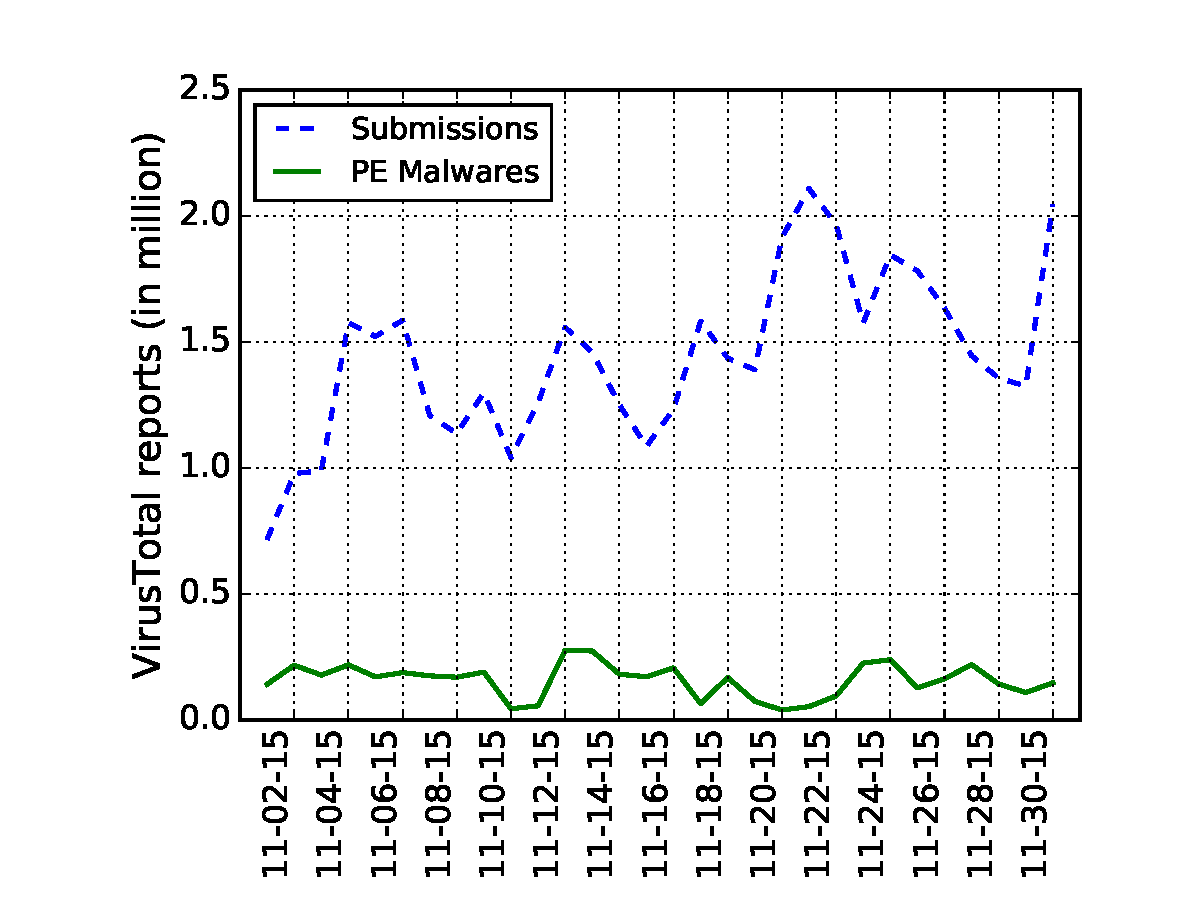
\includegraphics[width=2.5in]{figure/nov}
\mycaption{fig:subnum}{The number of files and malwares.}
{
The number of suspicious files and the number of malwares submitted to VirusTotal in November 2015. 
}
\end{center}
\vspace{-0.25in}
\end{figure}




In summary, this paper makes the following contributions:

\begin{itemize}

\item We are the first to collect mass data from the VirusTotal repository for large-scale malware study.
We collected and preprocessed files submitted to VirusTotal in November 2015 (Section~\ref{sec:meth}).
%and analyzed their general characteristics. 
%We find that most malware files are only submitted once to VirusTotal (Section~\ref{sec:meth}) 
%and that roughly 100-400 new malware families appear each day (Section~\ref{sec:temporal}). 

\item We studied the burstiness of malwares using a new 
cache-based malware prediction tool.
This tool achieves greater than 90\% prediction precision (Section~\ref{sec:temporal}). 

\item We observe that family distributions of malwares are highly skewed, 
\ie, some family has a huge amount of malwares while others only include a few malwares. 
Leveraging this observation, we built a hot malware family mining tool that identifies hot 
malware families (Section~\ref{sec:dist}).
%%% I don't understand this: using a constant number of counters

\item We identify several key research opportunities on top of the VirusTotal repository (Section~\ref{sec:oppo}). 

\end{itemize}


